\documentclass[12pt,a4paper]{article}
\usepackage{rmpackages}																% usual packages
\usepackage{rmtemplate}																% graphic charter
\usepackage{rmexocptce}																% for DS with cptce eval

%\cfoot{} 													% if no page number is needed
%\renewcommand\arraystretch{1.5}		% stretch table line height

\newcommand{\ritem}{\refstepcounter{enumi}\item[\color{bleu_f}\textbf{\theenumi .}]}

%%% Environnement fonction arduino
\newcounter{counterfunc}
\setcounter{counterfunc}{0}

\mdfdefinestyle{s_func}{%
	linecolor=arduino_keyword!,
	outerlinewidth=1pt,%
	frametitlerule=false,
	topline=true,
	bottomline=true,
	rightline=true,
	backgroundcolor=white,
	innertopmargin=8pt,
	roundcorner=0pt,
	nobreak=true,
	fontcolor=black
}
\newmdenv[style=s_func]{func_env}
\newenvironment{func}
{
	\refstepcounter{counterfunc}
	\begin{func_env}\textbf{Commande \thecounterfunc{}} :}
	{\end{func_env}
}

\begin{document}

\begin{header}
TP

Un diapason électronique
\end{header}

L'objectif de ce TP est de réaliser un diapason électronique en utilisant une carte équipée d'un microcontrôleur : la carte Arduino.

\begin{center}
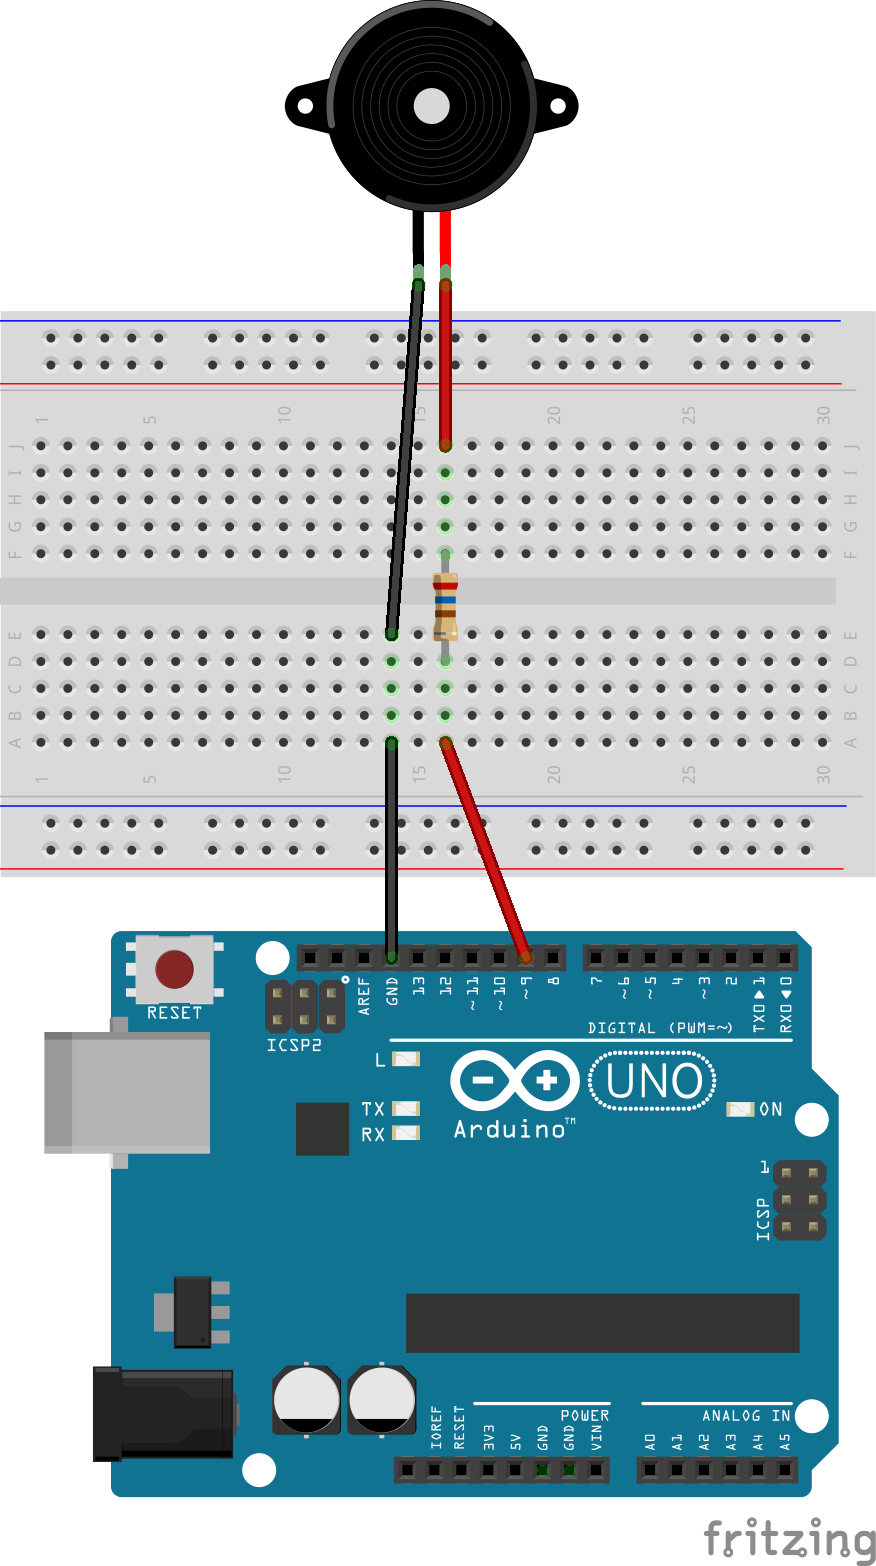
\includegraphics[scale=0.8, angle=-90]{fritzing/buzzer_bb.png}
\end{center}

\begin{enumerate}
\item \rea{}

Copier-coller tout le dossier \og TP Arduino \fg{} (Ordinateur \textrightarrow{} Ma classe \textrightarrow{} Documents en consultation \textrightarrow{} Physique-Chimie \textrightarrow{} TP Arduino) dans votre espace de travail personnel.
\end{enumerate}

\begin{enumerate}[resume]
\item \rea{}

Réaliser le montage électronique schématisé ci-dessus avec le matériel à votre disposition.

\item \rea{}

Connecter la carte à l'ordinateur avec le câble USB.
Ouvrir le programme \texttt{programme1} avec le logiciel Arduino.
Dans l'onglet \og Outil \fg{}, vérifier que le type de carte sélectionné est bien Arduino Uno et que le port sélectionné est bien COM1.
\end{enumerate}

\section*{La commande \texttt{tone}}

\begin{func}
\label{doc:tone}
\texttt{\textcolor{arduino_function}{tone}()}

\begin{itemize}
\item[•] Description : produit un signal périodique rectangulaire comme celui représenté ci-dessous.
\end{itemize}
\vspace{-1.5\baselineskip}
\begin{multicols}{2}
\begin{itemize}
\item[•] Syntaxe :

\texttt{\textcolor{arduino_function}{tone}(broche, freq, durée);}

{\color{red}\warning{} Ne pas oublier le \texttt{;} à la fin de la ligne !}

\item[•] Paramètres :

\texttt{broche} : numéro de la broche où est généré le signal ;

\texttt{freq} : fréquence du signal en hertz ;

\texttt{durée} : durée totale du signal en millisecondes.
\end{itemize}

\noindent


\begin{center}
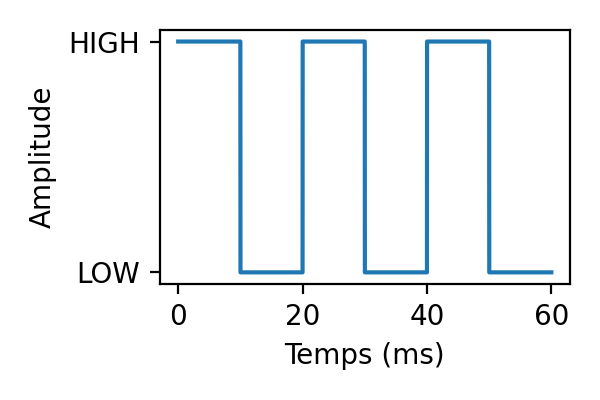
\includegraphics[scale=1]{images/tp_son_arduino_tone.png}
\end{center}

\end{multicols}

\end{func}

Un programme Arduino comprend au minimum deux fonctions (\texttt{setup} et \texttt{loop}) qui peuvent contenir plusieurs commandes.

\begin{enumerate}[resume]
\ritem \app{} \val{} \com{}

En utilisant la commande \texttt{tone}, compléter la fonction \texttt{setup} du \texttt{programme1} pour produire un son de fréquence \unit{440}{Hz} pendant \unit{1}{s} avec votre montage.
Compiler le programme et l'envoyer vers la carte en cliquant sur 
\includegraphics[height=0.75\baselineskip]{images/arduino_televerser.png} Téléverser.
Recopier la ligne ajoutée sur votre compte-rendu. 
\end{enumerate}
\begin{appel}
\rea{}

Appeler le professeur quand votre montage fonctionne ou en cas de difficulté.
\end{appel}

\begin{enumerate}[resume]
\ritem \anarai{} \rea{}

Déplacer la fonction \texttt{tone} ajoutée précédemment dans la fonction \texttt{loop}.
Téléverser le programme obtenu.
Pourquoi la fonction \texttt{loop} s'appelle-t-elle ainsi ?
\end{enumerate}

\section*{Et si \texttt{tone} n'existait pas ?}

\begin{multicols}{2}
\begin{func}
\texttt{\textcolor{arduino_function}{digitalWrite}()}
\begin{itemize}
\item[•] Description : place la broche dans l'état haut (\texttt{HIGH}) ou bas (\texttt{LOW}).
\item[•] Syntaxe :

\texttt{\textcolor{arduino_function}{digitalWrite}(broche, valeur);}
\item[•] Paramètres :

\texttt{broche} : numéro de la broche ;

\texttt{valeur} : \texttt{HIGH} ou \texttt{LOW}.
\end{itemize}
\end{func}

\begin{func}
\texttt{\textcolor{arduino_function}{delayMicroseconds}()}
\begin{itemize}
\item[•] Description : met le programme en pause pour une durée donnée.
\item[•] Syntaxe :

\texttt{\textcolor{arduino_function}{delayMicroseconds}(temps);}
\item[•] Paramètre :

\texttt{temps} : temps de pause en microsecondes. 
\end{itemize}
\end{func}
\end{multicols}

\begin{enumerate}[resume]
\ritem \rea{}

Calculer la période $T$ d'un son de fréquence $f = \unit{440}{Hz}$.
L'exprimer en microsecondes.

\textit{Rappel : $\unit{1}{\micro\second} = \unit{1\times 10^{-6}}{s}$.}

\ritem \app{} \anarai{} \com{}

Compléter et téléverser le \texttt{programme2} pour reproduire le signal généré par la fonction \texttt{tone} en utilisant uniquement les commandes \texttt{digitalWrite} et \texttt{delayMicroseconds}.
\end{enumerate}

\begin{appel}
\rea{}

Appeler le professeur quand votre montage fonctionne ou en cas de difficulté.
\end{appel}

\begin{enumerate}[resume]
\ritem \anarai{} \val{}

Proposer un protocole pour vérifier que le son ainsi produit a une fréquence de \unit{440}{Hz}.
\end{enumerate}

\begin{appel}
\anarai{}

Appeler le professeur pour lui présenter votre protocole avant de le mettre en pratique.
\end{appel}

\end{document}